\documentclass[xcolor=dvipsnames]{beamer}


\usetheme[
          showdate=true,                     % show the date on the title page
          alternativetitlepage=true,         % Use the fancy title page.
          titlepagelogo=general_figures/shell,              % Logo for the fir\
st page.
          ]{UMD}

%\usetheme{Rochester}

%\usepackage{beamerthemesplit}
\usepackage{xmpmulti}

\usepackage{booktabs}
\usepackage{graphicx,float,wrapfig, bbm}
\usepackage{amsfonts, bbold, comment}
\usepackage{mdwlist}
\usepackage{subfigure}
\usepackage{colortbl}

\usepackage{multirow}


\newcommand{\fsi}[2]{
\begin{frame}[plain]
\vspace*{-1pt}
\makebox[\linewidth]{\includegraphics[width=\paperwidth]{#1}}
\begin{center}
#2
\end{center}
\end{frame}
}

\newcommand{\abr}[1]{\textsc{#1} }
\newcommand{\pos}[1]{{\texttt{#1}}}
\newcommand{\e}[2]{\mathbb{E}_{#1}\left[ #2 \right] }
\newcommand{\ind}[1]{\mathbb{I}\left[ #1 \right] }
\newcommand{\ex}[1]{\mbox{exp}\left\{ #1\right\} }
\newcommand{\g}{\, | \,}
\newcommand{\citename}[1]{#1 }

\newcommand{\gfxs}[2]{
\begin{center}
	\includegraphics[width=#2\linewidth]{simtrans/#1}
\end{center}
}

\newcommand{\gfxq}[2]{
\begin{center}
	\includegraphics[width=#2\linewidth]{qb/#1}
\end{center}
}



%\usecolortheme{ucdblack}
\title[HCQA]{Cooperative and Competitive Machine Learning through Question Answering}
\author{ Jordan Boyd-Graber et al.}
\date{2017}

\institute[Maryland] % (optional, but mostly needed)
{University of Maryland}

\begin{document}

\frame{
\titlepage
\tiny
}

\fsi{qb/turing}{Turing Test: Definition of AI (Image from Wall Street
  International)}

\fsi{qb/jeopardy}{Question Answering as Yardstick (IBM)}

\fsi{qb/jennings_handshake}{Quiz Bowl as Question Answering ``Gold Standard''}

\begin{frame}{But First \dots a Recent History of Question Answering}

\begin{columns}
\column{.5\linewidth}
\gfxq{siri}{.8}
\column{.5\linewidth}
\begin{itemize}
  \item Reason across sentences
  \item Written by experts
  \item Compare/compete with humans
  \item Test uncertainty
  \item Advance science
\end{itemize}
\end{columns}

\end{frame}

\fsi{qb/squad}{SQuAD: Rajpurkar et al., 2016 (Reason)}

\fsi{qb/triviaqa}{TriviaQA: Joshi et al., 2017 (Experts)}

\fsi{qb/jeopardy}{IBM Watson: Buzzer Oddity}

\fsi{qb/human_reading}{SQuAD: Ignore Knowledge}

\fsi{qb/squad_2}{Test uncertainty (Rajpurkar et al., 2018)}

\begin{frame}
	\frametitle{Humans doing Incremental Classification}
	\begin{columns}

	\column{.5\linewidth}
	\begin{itemize}
		\item Game called ``quiz bowl''
		\item Two teams play each other
		\begin{itemize}
			\item Moderator reads a question
			\item When a team knows the answer, they signal (``buzz'' in)
			\item If right, they get points; otherwise, rest of the question is read to the other team
		\end{itemize}
		\item Hundreds of teams in the US alone
                \only<2>{\item Example \dots}
	\end{itemize}

	\column{.5\linewidth}
	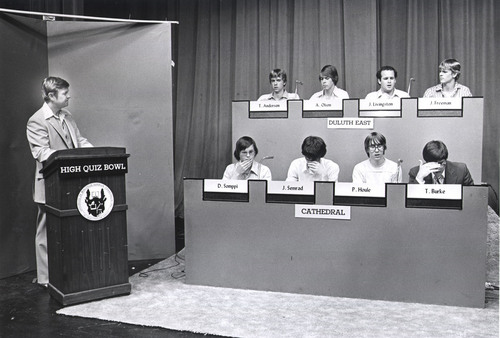
\includegraphics{qb/quizbowl}

	\end{columns}

\end{frame}

\begin{frame}[t]
  \frametitle{Sample Question}

\small
\only<2->{This man wrote a ballet in which 60 white nymphs perform the
  Rainbow Dance, so named because different colored lights are focused
  on them---\only<3->{that ballet Alethes and Iris was never produced
    because the theater manager was convinced it would cause a
    fire. He invented the first \only<4->{cow catcher and campaigned
      for passage of an act against "street nuisances" like outdoor
      musicians, who he claimed wasted a quarter of his life. He
      responded to \only<5->{William Whewell's statement that no
        scientific explanation of the universe was possible in his
        \only<6->{"Ninth Bridgewater Treatise," which attacked the
          eight previous treatises funded by the Earl of
          Bridgewater. He also wrote about the influence of
          aristocrats on science in his \only<7->{Reflections on the
            Decline of Science in England . This author of the memoir
            \only<8->{Passages From the Life of a Philosopher improved
              on \only<9->{Jacquard's invention of punched cards by
                proposing a device which incorporated an
                \only<10->{input, storage system, processor, control
                  unit, and output device. FTP, name this inventor of
                  the \only<11->{Analytic Engine and the Difference
                    Engine.}}}}}}}}}}

\only<12->{ {\bf Charles Babbage}}




\end{frame}


\begin{frame}[t]
	\frametitle{Sample Question}

        The Swiss-Italian architect Pietro Antonio Solari
        \only<2->{built several fortified towers in this city, which
          often vied for power with its northern rival Tver. A ruler
          of this city prevailed in the} \only<3->{Great Stand on the
          Ugra River. A prince from this city was nicknamed for
          winning a battle on the} \only<4->{Don river. Partly because
          a ruler of this city married} \only<5->{Sophia Palaiologina,
          the niece of the last Byzantine Emperor, this city styled
          itself the} \only<6->{``Third Rome'' after the fall of
          Constantinople. Another prince of this city stopped paying
          tribute to the} \only<7->{Mongols in 1476, ending the
          ``Tatar yoke.''} \only<8->{The Grand Duchy headquartered in
          this city came to an end in 1547 with the ascension of}
        \only<9->{ Ivan IV, who made it his capital. For 10 points,
          name this city where Ivan III renovated the
          Kremlin,} \only<10->{the capital of Russia.}\\
        \vspace{.5cm} \only<11->{ {\bf Moscow} (Moskva / Muscovy)}

\end{frame}


\begin{frame}
	\frametitle{Question Structure Enables Compeition}

	\begin{columns}
		\column{.5\linewidth}

		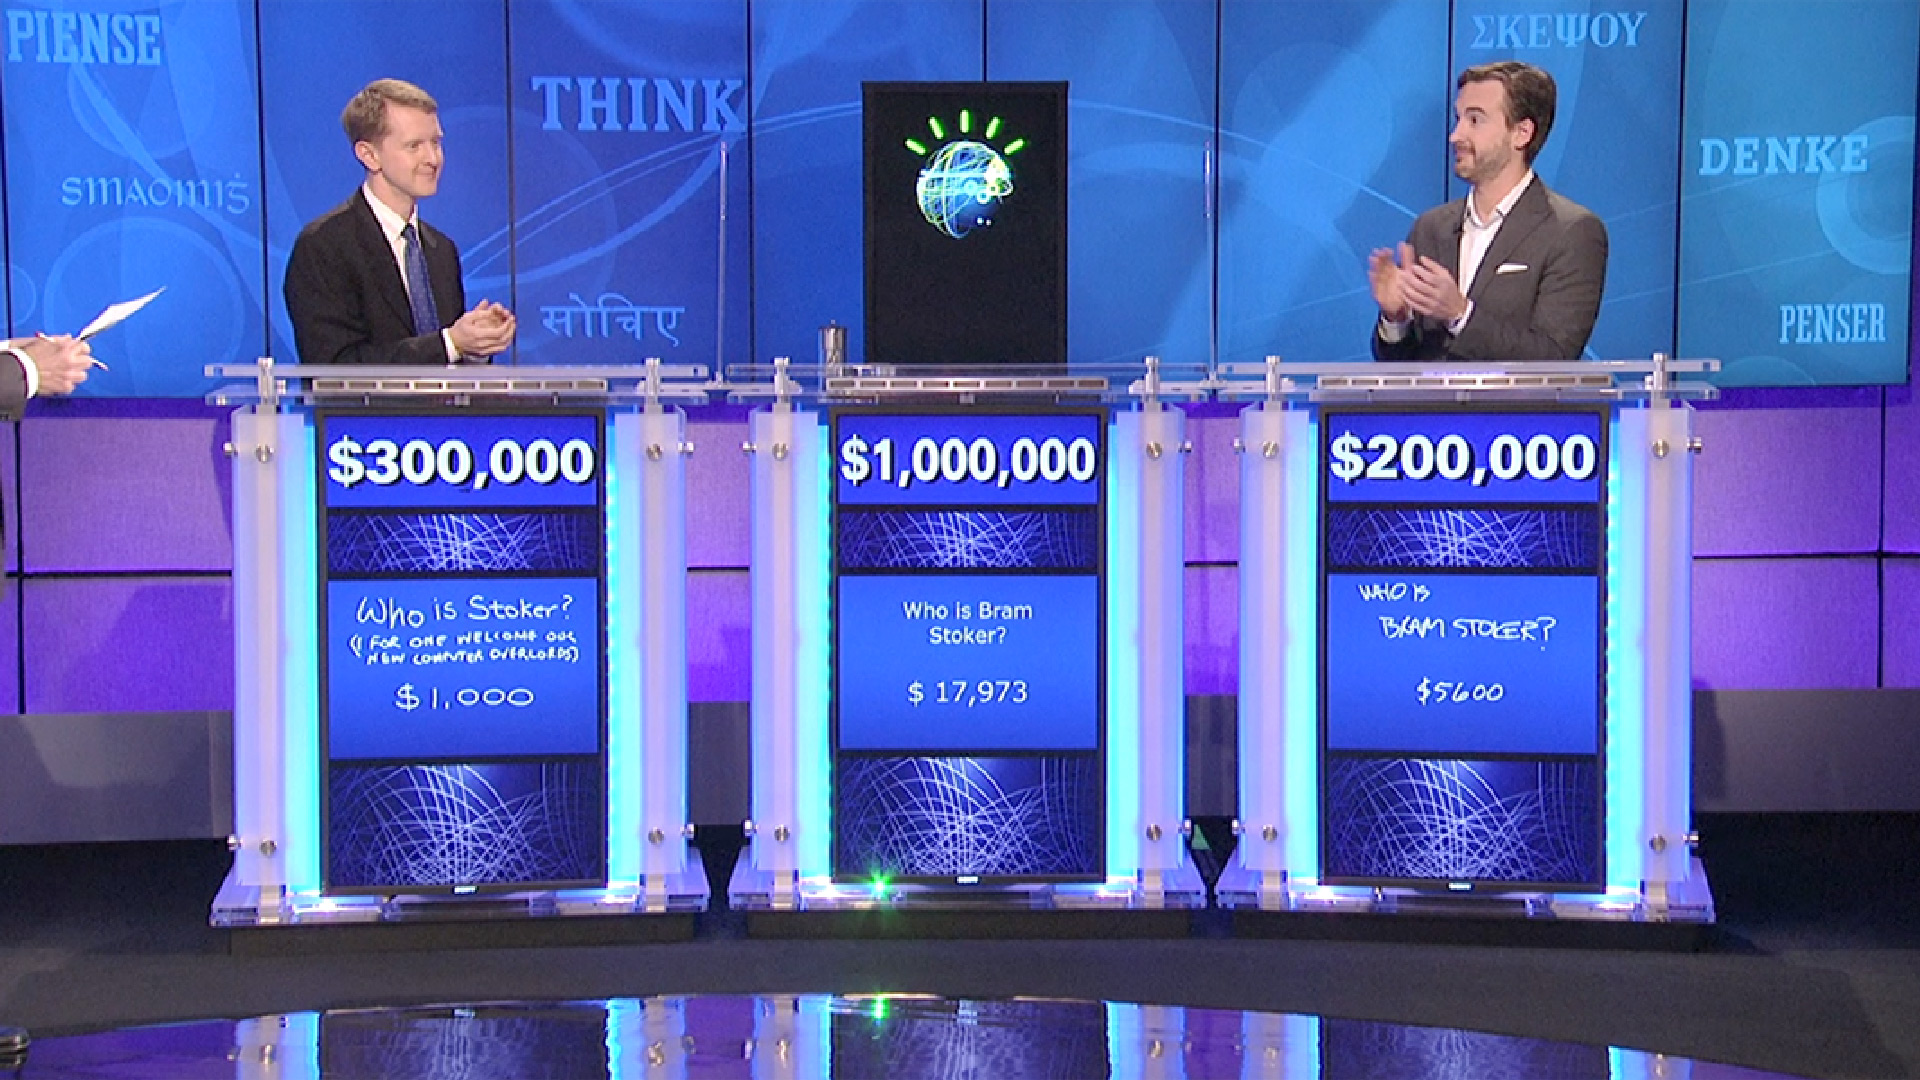
\includegraphics[width=1.0\linewidth]{qb/jeopardy}


		\column{.5\linewidth}
		\begin{itemize}
                        \item Watson must decide to answer {\bf once}, after
                          complete question
                        \item Quiz Bowl: decide after each word
                        \item Obscure clues at start, easy at end
                        \item ``Gold standard'' in trivia community
		\end{itemize}

	\end{columns}

\end{frame}

\begin{frame}{Checklist}

\begin{itemize}
  \item Reason across sentences\only<2->{: question and source}
  \item Written by experts\only<3->{: trivia community}
  \item Compare/compete with humans\only<4->{: by design}
  \item Test uncertainty\only<5->{: by design}
  \item \alert<6>{Advance science} \only<6>{(More later)}
\end{itemize}

\end{frame}


\begin{frame}{How to approach this problem \dots}

    \only<1>{
  \begin{columns}
    \column{.5\linewidth}
    \gfxq{guess}{0.8}
    \column{.5\linewidth}
    \gfxq{buzzer}{0.8}
  \end{columns}
}
\only<2>{
   \gfxq{guess}{0.5}
}
\end{frame}



\begin{frame}{}

  \begin{columns}
    \column{.4\linewidth}
    \begin{center}
        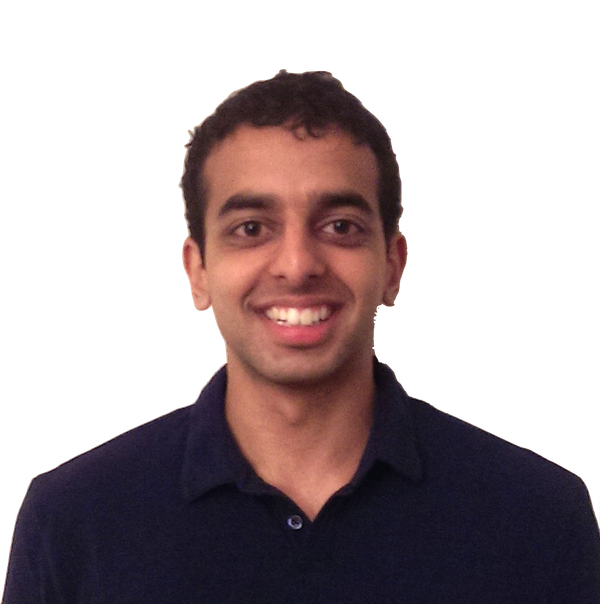
\includegraphics[width=0.8\linewidth]{general_figures/mohit}
        \end{center}
    \column{.6\linewidth}
        \begin{block}{ {\bf \href{http://cs.colorado.edu/~jbg//docs/2014_emnlp_qb_rnn.pdf}{A Neural Network for Factoid Question Answering over Paragraphs}}}
\underline{\href{http://cs.umd.edu/~miyyer/}{Mohit Iyyer}}, {\bf Jordan Boyd-Graber}, Leonardo Claudino, Richard Socher, and Hal {Daum\'{e} III}.  \emph{Empirical Methods in Natural Language Processing}, 2014
        \end{block}

        \begin{block}{ {\bf \href{file:///Users/jbg/public_html/docs/2015_acl_dan.pdf}{Deep Unordered Composition Rivals Syntactic Methods for Text Classification}}}
\underline{\href{http://cs.umd.edu/~miyyer/}{Mohit Iyyer}}, Varun
Manjunatha, {\bf Jordan Boyd-Graber} and Hal {Daum\'{e} III}.  \emph{Empirical Methods in Natural Language Processing}, 2014
        \end{block}

  \end{columns}
\end{frame}
\begin{frame}{Vector Space Model}

  \only<1>{\gfxq{unigram_models_0}{.8}}
  \only<2>{\gfxq{unigram_models_1}{.8}}
  \only<3>{\gfxq{unigram_models_2}{.8}}
  \only<4>{\gfxq{unigram_models_3}{.8}}
  \only<5>{\gfxq{unigram_models_4}{.8}}
  \only<6>{\gfxq{unigram_models_5}{.8}}
  \only<7>{\gfxq{unigram_models_6}{.8}}
  \only<8>{\gfxq{unigram_models_7}{.8}}
  \only<9>{\gfxq{unigram_models_8}{.8}}


\end{frame}



\begin{frame}{How can we do better?}

  \begin{itemize}
    \item Use relationship between questions (``China'' and
      ``Taiwan'')
    \item Use learned features and dimensions, not the words we start with
  \end{itemize}

\end{frame}



\begin{frame}{Deep Averaging Networks}

  \only<1>{\gfxq{dan_1}{.8}}
  \only<2>{\gfxq{dan_2}{.6}}
  \only<3>{\gfxq{dan_3}{.6}}
  \only<4>{\gfxq{dan_4}{.6}}

\end{frame}




\begin{frame}{Training}

  \begin{columns}
    \column{.5\linewidth}
      \begin{itemize}
        \item Initialize embeddings from \textsc{word2vec}
        \item Randomly initialize composition matrices
        \item Update using \textsc{warp}
          \begin{itemize}
            \item Randomly choose an instance
            \only<2->{\item Look where it lands}
            \only<4->{\item Has a correct answer}
            \only<5->{\item Wrong answers may be closer}
            \only<6->{\item Push away wrong answers
            \item Bring correct answers closer}
          \end{itemize}
      \end{itemize}

    \column{.5\linewidth}

      \only<1>{\gfxq{warp_training_5}{.8}}
      \only<2>{\gfxq{warp_training_4}{.8}}
      \only<3>{\gfxq{warp_training_3}{.8}}
      \only<4>{\gfxq{warp_training_2}{.8}}
      \only<5>{\gfxq{warp_training_1}{.8}}
      \only<6>{\gfxq{warp_training_0}{.8}}
  \end{columns}

\end{frame}

\begin{frame}{Performance (Sentiment Analysis)}


\footnotesize
\begin{center}
\begin{tabular}{cccccc}
\toprule
Model & RT & SST & SST & IMDB & Time \\
& & fine & bin & & (s)\\
\midrule
\footnotesize DAN & 80.3 & 47.7 & 86.3 & 89.4 & 136\\
\midrule
\footnotesize NBOW-RAND & 76.2 & 42.3 & 81.4 & 88.9 & 91 \\
\footnotesize NBOW & 79.0 & 43.6 & 83.6 & 89.0 & 91 \\
\footnotesize BiNB & --- & 41.9 & 83.1 & --- & ---\\
\footnotesize NBSVM-bi & 79.4 & --- & --- & 91.2 & ---\\
\midrule
\footnotesize RecNN$^*$ & 77.7 & 43.2 & 82.4 & --- & --- \\
\footnotesize RecNTN$^*$ & --- & 45.7 & 85.4 & --- & --- \\
\footnotesize DRecNN & --- & 49.8 & 86.6 & --- & 431\\
\footnotesize TreeLSTM & --- & \bf 50.6 & 86.9 & --- & --- \\
\footnotesize DCNN$^*$ & --- & 48.5 & 86.9 & 89.4 & ---\\
\footnotesize PVEC$^*$ & --- & 48.7 & 87.8 & \bf 92.6 & --- \\
\footnotesize CNN-MC & \bf 81.1 & 47.4 & \bf 88.1 & --- & 2,452 \\
\footnotesize WRRBM$^*$ & --- & --- & --- & 89.2 & ---\\
\bottomrule
\end{tabular}
\end{center}
\end{frame}


\begin{frame}{Embedding}

  \gfxq{embedding}{1.0}

\end{frame}


\begin{frame}{How to approach this problem \dots}

    \only<1>{
  \begin{columns}
    \column{.5\linewidth}
    \gfxq{guess}{0.8}
    \column{.5\linewidth}
    \gfxq{buzzer}{0.8}
  \end{columns}
}
\only<2>{
   \gfxq{buzzer}{0.5}
}
\end{frame}


\begin{frame}{}

  \begin{columns}
    \column{.5\linewidth}
        
\includegraphics[width=0.7\linewidth]{general_figures/hehe}
    \column{.5\linewidth}
        \begin{block}{{\bf
              \href{http://cs.colorado.edu/~jbg//docs/qb_emnlp_2012.pdf}{Besting
                the Quiz Master: Crowdsourcing Incremental
                Classification Games}}}

          {\bf Jordan Boyd-Graber}, He He, and Hal {Daum\'{e} III}. \emph{Empirical Methods in Natural Language Processing}, 2012
        \end{block}

        \begin{block}{{\bf
              \href{http://www.cs.colorado.edu/~jbg/docs/2016_icml_opponent.pdf}{Opponent Modeling in Deep Reinforcement Learning}}}

          He He, {\bf Jordan Boyd-Graber}, Kevin Kwok, and Hal
          {Daum\'{e} III}. \emph{International Conference of Machine Learning}, 2016
        \end{block}

  \end{columns}
\end{frame}


\begin{frame}
\frametitle{Interface}

\begin{columns}

	\column{0.5\linewidth}

	\begin{center}
		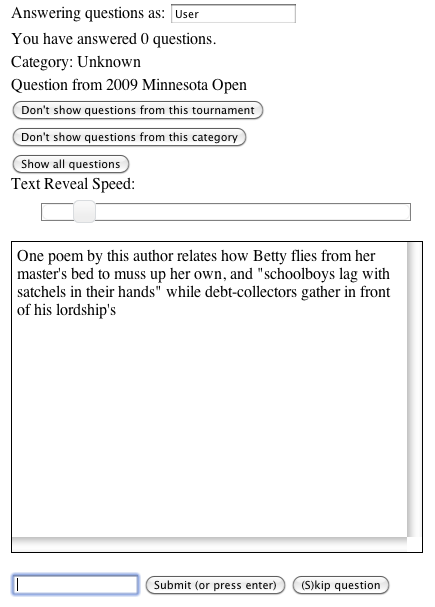
\includegraphics[width=0.8\linewidth]{qb/screenshot}
	\end{center}

	\column{0.5\linewidth}


	\only<2>{
	\begin{itemize}
		\item 7000 questions: first day
		\item 43000 questions: two weeks
		\item 461 unique users
                \item Imitated \dots
	\end{itemize}
        \gfxq{protobowl}{.8}
	}



\end{columns}
\end{frame}





\begin{frame}{How can this fail?}

  \only<1>{\gfxq{opponent_fail1}{.8}}
  \only<2>{\gfxq{opponent_fail2}{.8}}
  \only<3>{\gfxq{opponent_fail3}{.8}}
  \only<4>{\gfxq{opponent_fail4}{.8}}
  \only<5>{\gfxq{opponent_fail5}{.8}}
  \only<6>{\gfxq{opponent_fail6}{.8}}
  \only<7>{\gfxq{opponent_fail7}{.8}}

\end{frame}

\begin{frame}{Can we do better?}

  \only<1>{\gfxq{dqn_overview2}{.8}}
  \only<2>{\gfxq{dqn_overview3}{.8}}
  \only<3>{\gfxq{dqn_overview4}{.8}}

\end{frame}

\begin{frame}{Not all opponents are equal}

  \gfxq{player_profile}{.9}

  \pause
  Varies by category!

\end{frame}

\begin{frame}{Comparing Models}

  \begin{itemize}
    \item Single-Player
    \item Deep Q-Network (DQN): World=Opponent~\cite{mnih-15}
      \begin{itemize}
        \item Learn representation of state to estimate $Q$-function
        \item Generalization of regression-based methods
        \item Similar to our representation of content
      \end{itemize}
    \item Deep Reinforcement Opponent Network (DRON)
  \end{itemize}

\end{frame}


\begin{frame}{Many models, choose which: DRON-MoE}

  \only<1>{\gfxq{dron-moe}{.8}}
  \only<2>{\gfxq{dron-moe2}{.8}}

\end{frame}

\begin{frame}{Reward}

  \gfxq{dqn_results}{.5}

\end{frame}

\begin{frame}{Reward: Closer Look}

  \only<1>{\gfxq{reward1}{.8}}
  \only<2>{\gfxq{reward2}{.8}}
  \only<3>{\gfxq{reward3}{.8}}
  \only<4>{\gfxq{reward4}{.8}}
\end{frame}

\begin{frame}{Experiment 1}

		\begin{columns}
			\column{.25\linewidth}
				\gfxq{colby_jeo}{1.0}
                                Colby Burnett:
                                \$375,000
			\column{.25\linewidth}
				\gfxq{ben_jeo}{1.0}
                                Ben Ingram:
                                \$427,534
			\column{.25\linewidth}
				\gfxq{alex_jeo}{1.0}
                                Alex Jacobs: \$151,802
			\column{.25\linewidth}
				\gfxq{kristin_jeo}{1.0}
                                Kristin Sausville: \$95,201
		\end{columns}

                \pause


                \begin{center}
                End result: 200-200 tie!
                \end{center}

\end{frame}

\fsi{qb/hsnct1}{}
\fsi{qb/jennings}{23. October 2015, Seattle}
\fsi{qb/jennings_handshake}{300-160}
\fsi{qb/nasat}{Humans 345-145}
\fsi{qb/hsnct_2017}{Computer 260-215}



\begin{frame}{Where we have problems}

\only<1-2>{
\begin{block}{Out of Date}
Although he won the California primary in 2000, he distanced himself
from fellow reform presidential candidate Pat Buchanan by comparing
him to Attila the Hun. After being called a jackass, he prompted
Lindsey Graham to destroy his phone by giving out his number during a
speech. The slogan (*) Make America Great Again has been used by this
politician, who claimed he didn't like people who were captured as a
slight to John McCain and kicked off his 2016 presidential bid with
some inflammatory remarks about Mexicans. For 10 points, name this
Republican candidate and real estate mogul.
\end{block} }
\only<2>{{\bf Chris Christie?}}

\only<3-4>{
\begin{block}{Out of Touch}
  This singer recently cancelled the Great Escape Tour, and, in one
  song, she claims that she will be ``Eating crumpets with the sailors
  / On acres without the neighbors.'' She collaborated with Jennifer
  (*) Hudson on the song ``Trouble,'' which was issued in her album
  update Reclassified. This artist of ``Change Your Life'' was
  inspired by scenes from the movie Clueless to make the music video
  for a song in which she collaborated with Charli XCX. For 10 points,
  name this Australian rapper whose album The New Classic contained
  ``Fancy.''
\end{block} }
\only<4>{{\bf Bruce Springsteen?}}

\end{frame}




\begin{frame}{Matching Entites Across Sentences}

\begin{block}{\only<2->{Magic Flute}}

    At its premiere, \alert<3>{the librettist of this opera} portrayed
    \alert<4>{a character who asks for a glass of wine with his dying wish}. \alert<4>{That
    character} in this opera is instructed to ring some bells to summon
    his love. At its beginning, \alert<5>{a man} who claims to have killed a (*)
    serpent has a padlock put on \alert<5>{his} mouth because of \alert<5>{his} lying. The
    plot of this opera concerns a series of tests that \alert<5>{Tamino} must
    undergo to rescue Tamina from Sorastro. For 10 points, name this
    Wolfgang Mozart opera titled for \alert<6>{an enchanted woodwind instrument}.
\end{block}



\only<3-4>{{\bf Not all references are named (\alert<3>{Emanuel
      Schikaneder}, \alert<4>{Papageno})}}
\only<5>{Need to be able to match pronouns across sentences (or have
  deep world knowledge)}
\only<6>{Requires semantic knowledge}
\end{frame}



\begin{frame}[plain]
\gfxq{seattle_crowd}{.5}
\gfxq{chicago_crowd}{.5}
\end{frame}

\fsi{qb/boring_dot_products}{}

\fsi{simtrans/centaur-chess}{Centaur Chess}

\begin{frame}{Measuring Interpretability}

  \only<1>{\gfxq{qb_centaur_1}{.9}}
  \only<2>{\gfxq{qb_centaur_2}{.9}}
  \only<3>{\gfxq{qb_centaur_3}{.9}}
  \only<4>{\gfxq{qb_centaur_6}{.9}}

\end{frame}


\fsi{qb/augment/screenshot_all}{Interface}

\fsi{qb/augment/screenshot_guesses}{Guesses}

\fsi{qb/augment/screenshot_highlight}{Highlight}

\fsi{qb/augment/screenshot_evidence}{Evidence}

\fsi{qb/augment/coefs}


\begin{frame}{Improvement through Reinforcement Learning}

  \only<1>{\gfxq{rl_centaur_2}{.9}}
  \only<2>{\gfxq{rl_centaur_3}{.9}}
  \only<3>{\gfxq{rl_centaur_4}{.9}}
  \only<4>{\gfxq{rl_centaur_5}{.9}}
  \only<5>{\gfxq{rl_centaur_6}{.9}}

\end{frame}

\begin{frame}{Can we improve QA systems?}

\begin{columns}
  \column{.6\linewidth}
     \gfxq{trick/pyramid}{.9}
     \column{.4\linewidth}
     \begin{itemize}
       \item Questions should be pyramidal
       \item But for whom?
         \begin{itemize}
           \item Quotes
           \item Reusing clues
         \end{itemize}
         \item Adversarial writing
         \item Improve questions
     \end{itemize}
\end{columns}
\end{frame}

\fsi{qb/trick/revealed_accuracy}{}

\begin{frame}{}

  \begin{columns}
    \column{.4\linewidth}
        
\includegraphics[width=0.8\linewidth]{general_figures/hehe} \\
        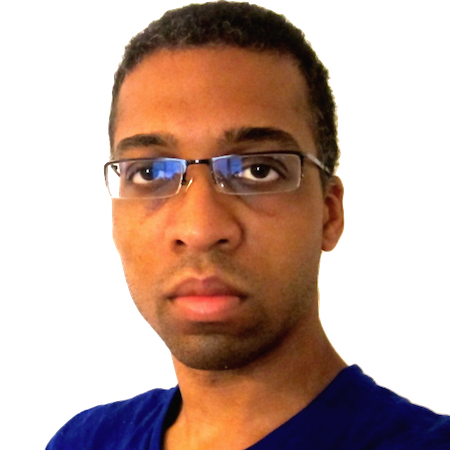
\includegraphics[width=0.8\linewidth]{general_figures/alvin}
    \column{.6\linewidth}

        \begin{block}{ {\bf \href{http://umiacs.umd.edu/~jbg//docs/2015_emnlp_rewrite.pdf}{Syntax-based Rewriting for Simultaneous Machine Translation}}}
He He, Alvin Grissom II, {\bf Jordan Boyd-Graber}, and Hal {Daum\'{e} III}.  \emph{Empirical Methods in Natural Language Processing}, 2015
        \end{block}

        \begin{block}{ {\bf \href{http://umiacs.umd.edu/~jbg/docs/2016_naacl_interpretese.pdf}{Interpretese vs. Translationese: The Uniqueness of Human Strategies in Simultaneous Interpretation}}}
He He, {\bf Jordan Boyd-Graber}, and Hal {Daum\'{e} III}.
\emph{North American Association for Computational Linguistics}, 2016
        \end{block}

  \end{columns}


\end{frame}

\begin{frame}{Simultaneous Interpretation is Hard!}

  \begin{columns}
    \column{.5\linewidth}
  \begin{itemize}
    \item Exhausting for humans
    \item Computers not trusted
    \item Differential strengths
    \item Same word-by-word characteristic
  \end{itemize}

  \column{.5\linewidth}
 \gfxs{computer-interpreter}{1.0}
 \end{columns}
\end{frame}

\begin{frame}{How we could translate a sentence}

\only<1>{\gfxs{example_3}{.9}}
\only<2>{\gfxs{example_4}{.9}}
\only<3>{\gfxs{example_5}{.9}}
\only<4>{\gfxs{example_6}{.9}}
\only<5>{\gfxs{example_7}{.9}}
\only<6>{\gfxs{example_8}{.9}}
\only<7>{\gfxs{example_9}{.9}}
\only<8>{\gfxs{example_10}{.9}}
\only<9>{\gfxs{example_11}{.9}}
\only<10>{\gfxs{example_12}{.9}}
\only<11>{\gfxs{example_13}{.9}}
\only<12>{\gfxs{example_14}{.9}}
\only<13>{\gfxs{example_15}{.9}}
\only<14>{\gfxs{example_16}{.9}}
\only<15>{\gfxs{example_17}{.9}}
\only<16>{\gfxs{example_18}{.9}}
\only<17>{\gfxs{example_19}{.9}}
\end{frame}

\begin{frame}{Human-Computer Question Answering}

  \begin{itemize}
    \item Pit machine learning algorithms against humans
    \item Fun task for human participants
    \item Good system for discriminating depth and confidence of
      algorithms
    \item Knowledge and language comprehension needed to do well
    \item Simple approaches work well if you have the whole question
    \item Good competition for QA systems
      \pause
    \item Can get much harder
     \begin{itemize}
       \item Speech
       \item Specialized knowledge
       \item Adversarial authoring
     \end{itemize}
  \end{itemize}

\end{frame}


\begin{frame}{Stay tuned \dots}

  \begin{itemize}
    \item Clearly dominating computer team
    \item Playing against human team December 8 in Long Beach
    \item Infrastructure for future events / courses
      \begin{itemize}
        \item Build it break it fix it
        \item HS / college competitions (DC area first)
      \end{itemize}
  \end{itemize}

\end{frame}





\begin{frame}{Find out More!}

		\begin{itemize}
			\item Code: \url{http://github.com/Pinafore/qb}
                        \item Shared Task \url{hcqa.boydgraber.org}
		\end{itemize}

\end{frame}

% \begin{frame}{Come to UMD}

% \begin{columns}
% 	\column{.5\linewidth}
%         \only<1>{
%         	\begin{center}
% 		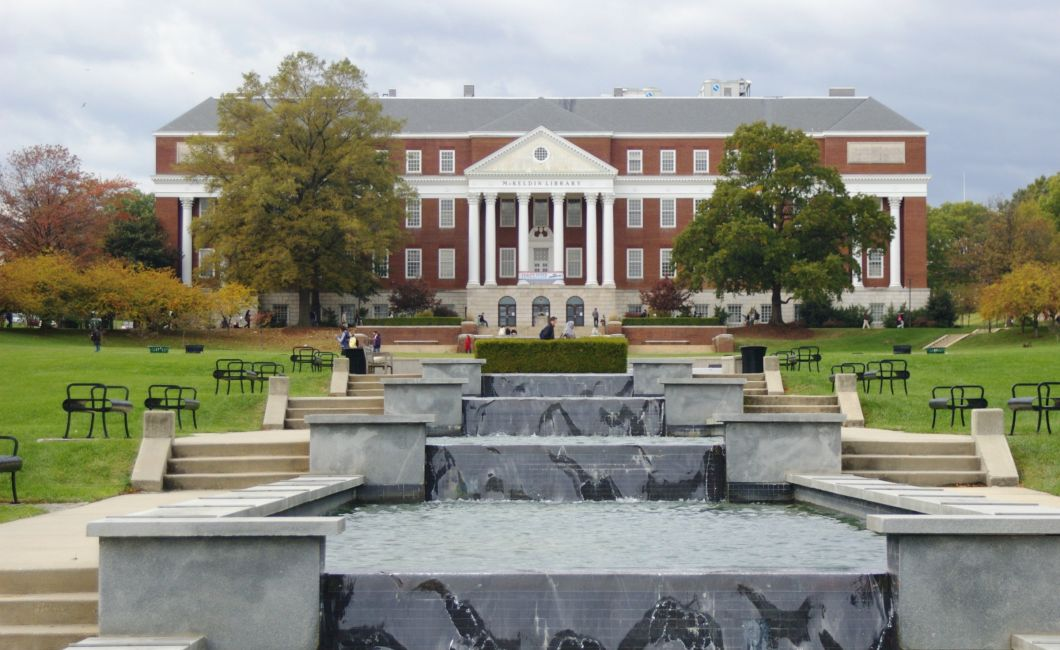
\includegraphics[width=.9\linewidth]{umd/umd} \\
% 		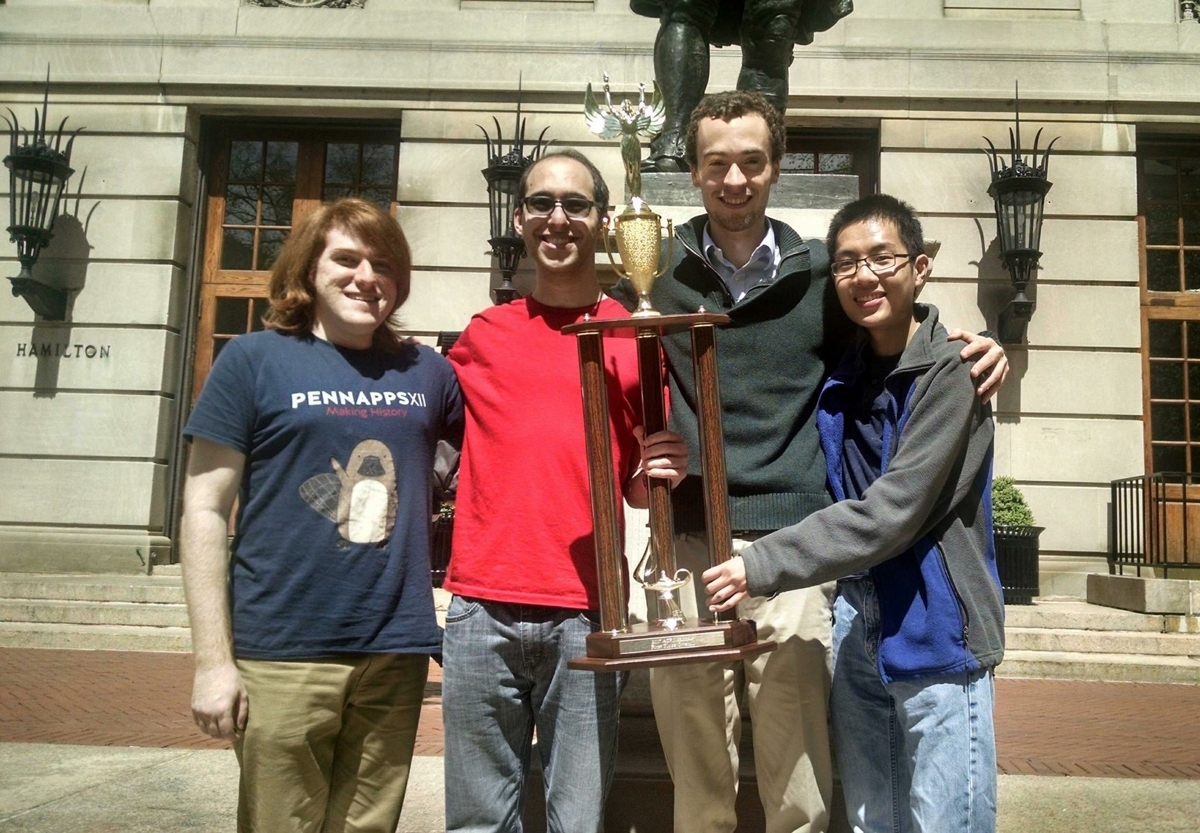
\includegraphics[width=.9\linewidth]{umd/qb_team}
% 	\end{center}
%               }
% 	\column{.5\linewidth}
% 		\begin{itemize}
%                 \item Looking for undergrads/grads/interns
%                 \item A great place for natural language
%                   processing and machine learning
%                 \item Not too shabby at quiz bowl either
% 		\end{itemize}
% \end{columns}

% \end{frame}

\frame{
  \frametitle{But wait, there's more!}

  \vspace{-.5cm}

\begin{columns}



  \column{.5\linewidth}

   \begin{block}{Computational Social Science}
     \centering
     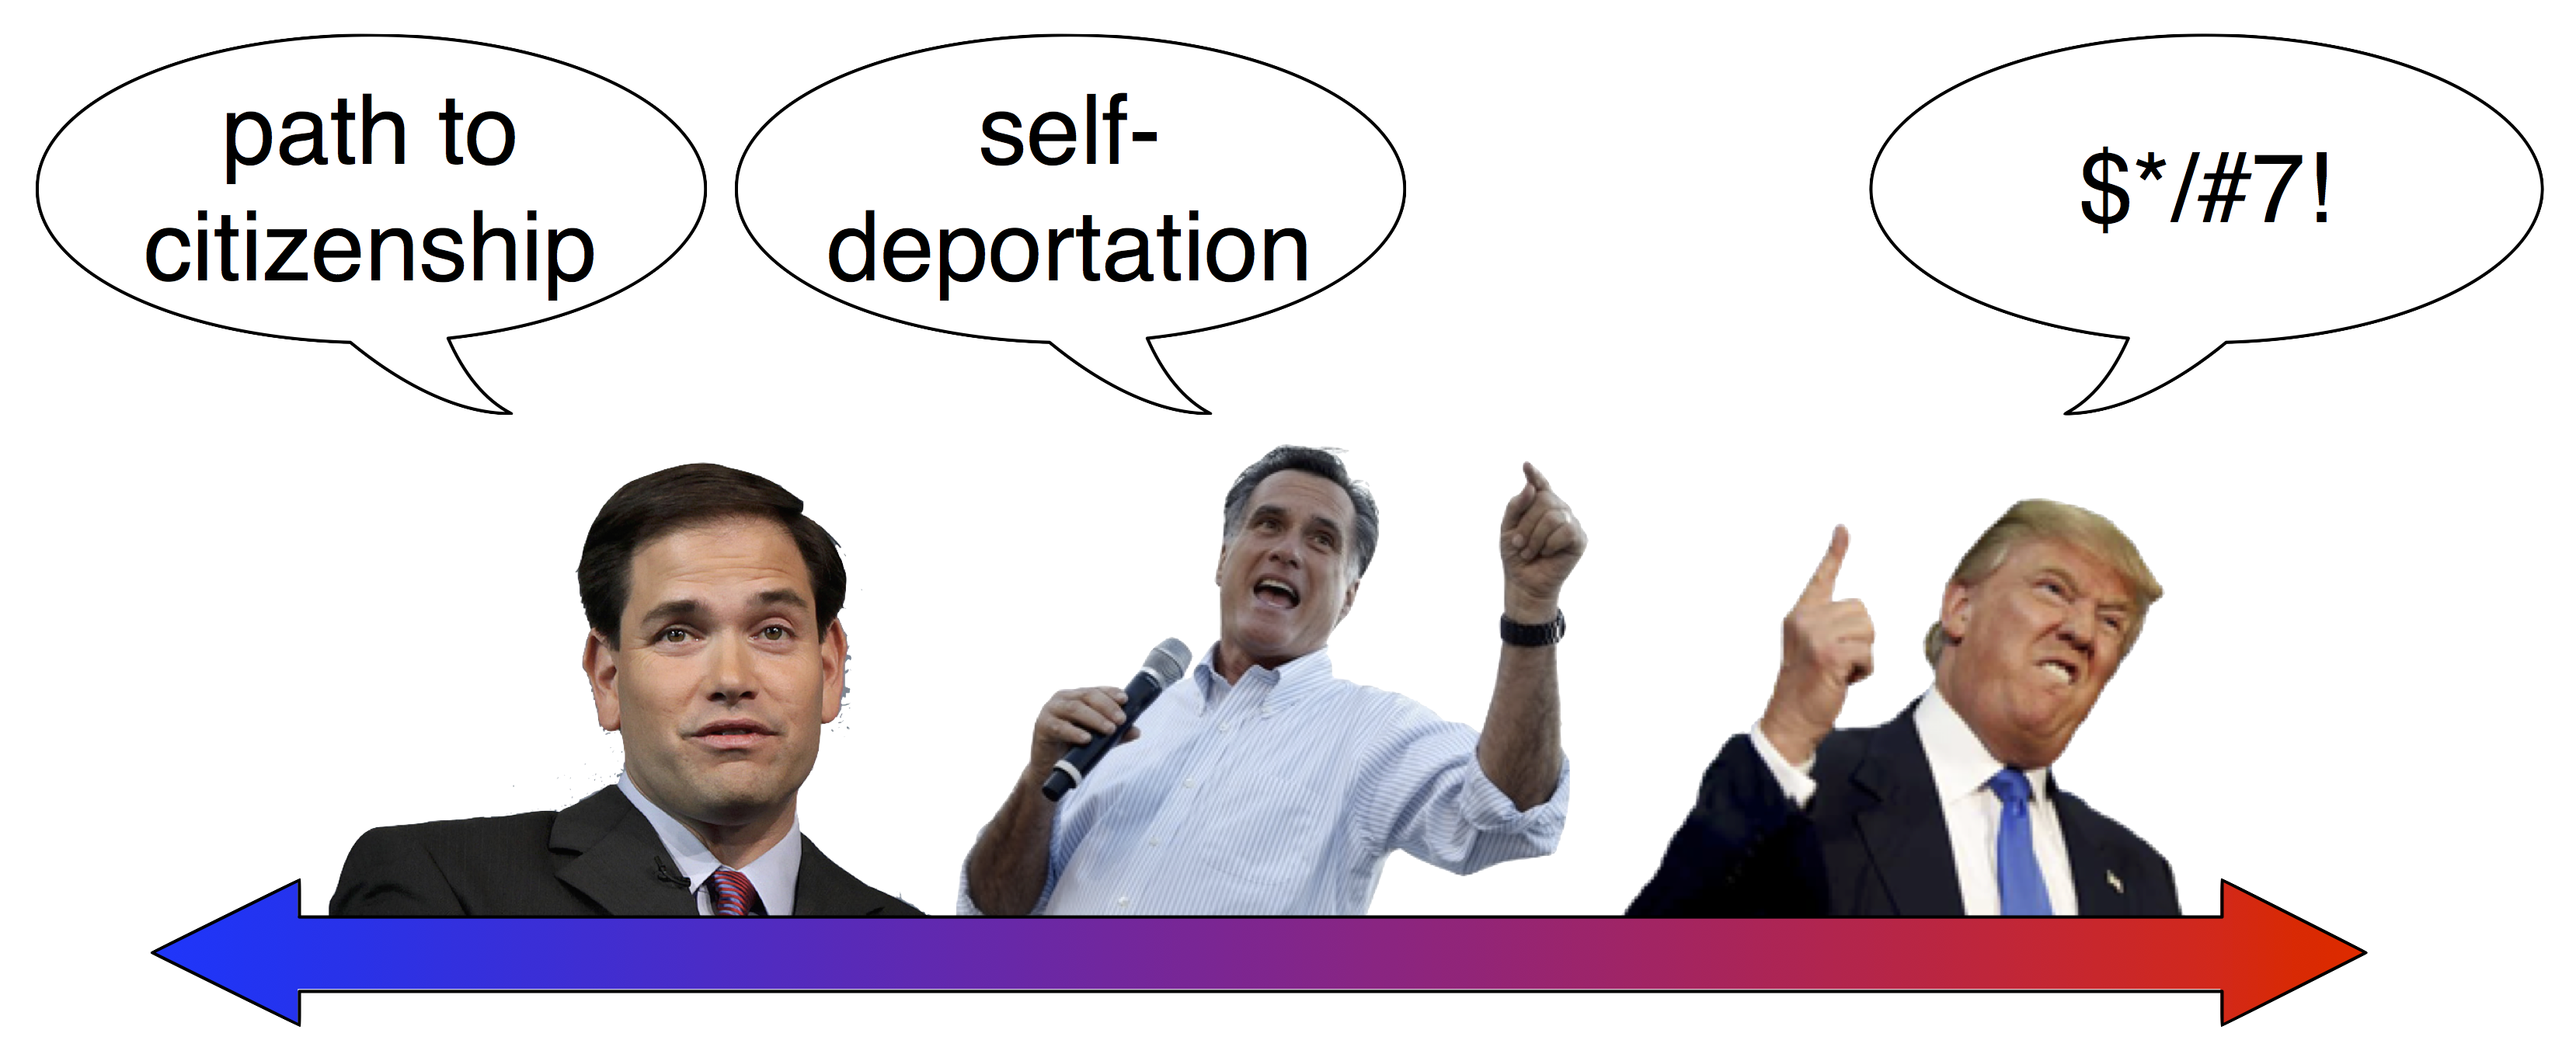
\includegraphics[width=0.9\linewidth]{teaparty/figures/framing} \\
     \cite{nguyen-13b,nguyen-15}
   \end{block}


    \begin{block}{Interactive Machine Learning}
     \centering
        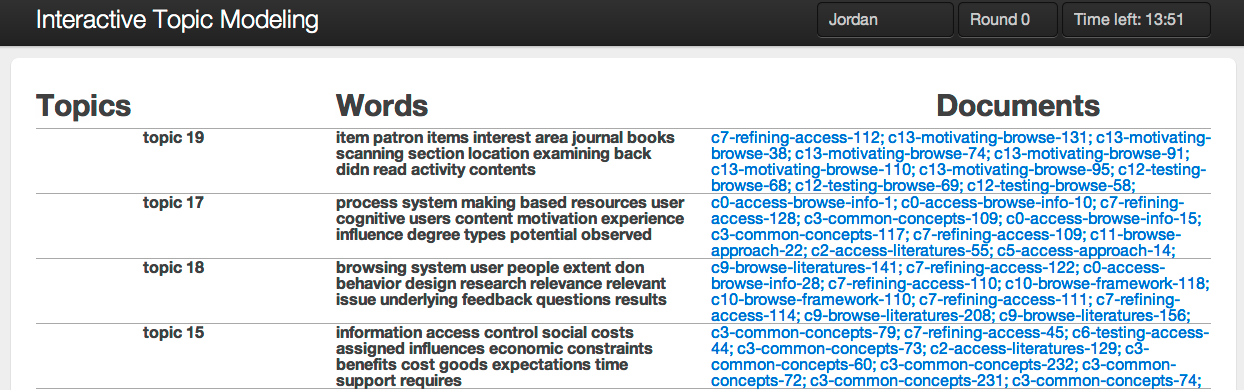
\includegraphics[width=0.4\linewidth]{interactive_topic_models/new_interface} \\
       \cite{Smith-17,Poursabzi-16}
    \end{block}


  \column{.5\linewidth}


    \begin{block}{Multilingual Topic Models}
      \begin{center}
        \begin{large}
          $p_{\mbox{topic}}(e | f)$ \\
         \end{large}
      \cite{eidelman-12,hu-14}
       \end{center}
    \vspace{-.3cm}
    \end{block}


    \begin{block}{Sentiment / Internal State}
    \centering
        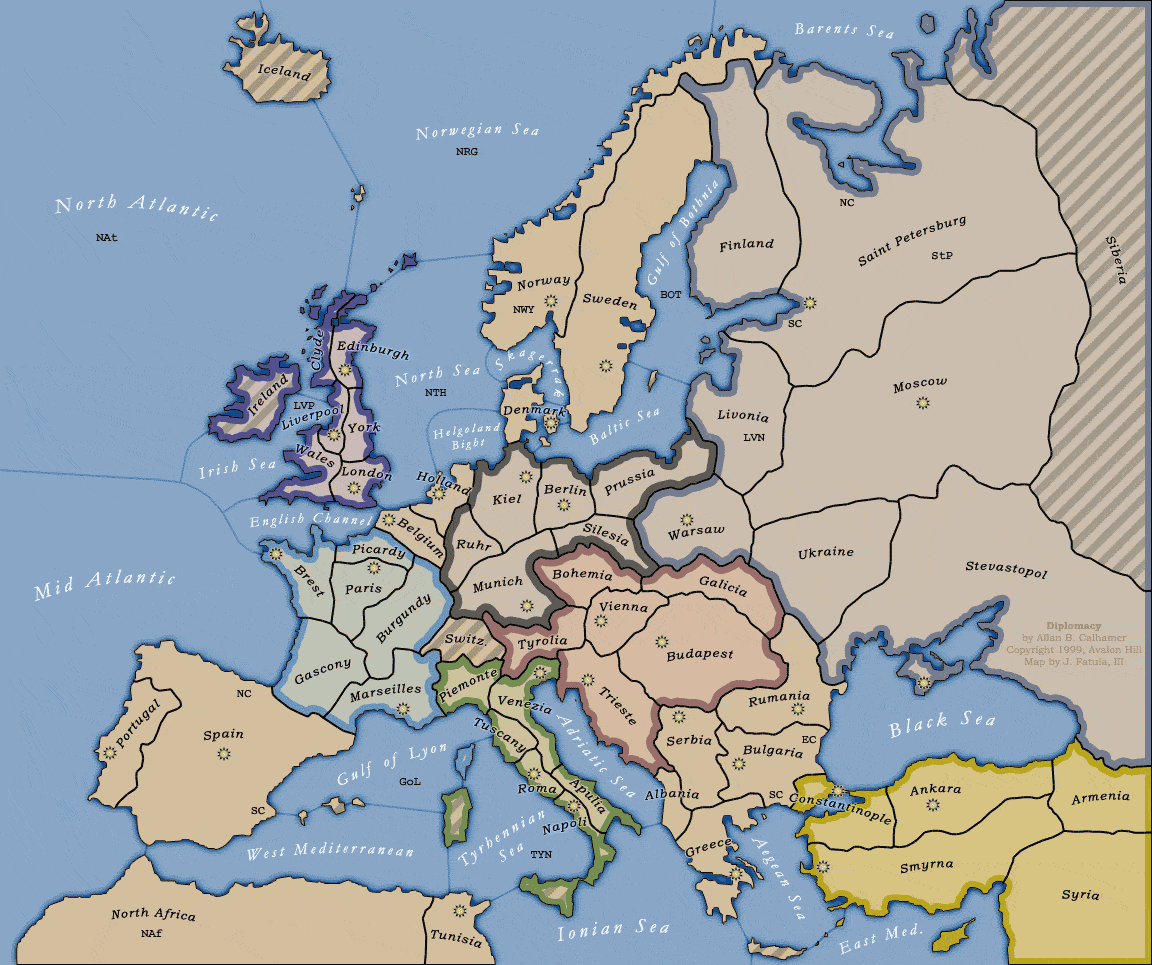
\includegraphics[width=0.4\linewidth]{general_figures/diplomacy} \\
        \cite{niculae-15,sayeed-12,boyd-graber-10}
    \end{block}




\end{columns}

}




\frame{

	\frametitle{Thanks}

        \begin{block}{Collaborators (not listed on previous slides)}
          Anupam Guha (Maryland), Manjhunath Ravi (Colorado), Danny Bouman (UMD UG),
          Stephanie Hwa (UMD UG), Yogarshi Vyas (UMD), Larry Davis
          (UMD), Naho Orita (Tohoku), Snigdha Chaturvedi (UMD), Varun
          Manjunatha (UMD), Srijan Kumar (UMD), Vlad Niculae
          (Cornell), Cristian Danescu-Niculescu-Mizil (Cornell),
          Richard Socher (Salesforce), Leonardo Claudino (UMD)
        \end{block}

	\begin{columns}

	\column{.5\linewidth}
        \begin{block}{Funders}
        \begin{center}
          
\includegraphics[width=0.4\linewidth]{general_figures/nsf}
       \end{center}
        \end{block}

	\column{.5\linewidth}
        \begin{block}{Supporters}
        	\gfxq{naqt}{.4}
        \end{block}

        \end{columns}
}

\begin{frame}{References}
\bibliographystyle{style/acl}
\tiny
\bibliography{bib/journal-full,bib/jbg}
\end{frame}




\begin{frame}[plain]


\only<4->{\vspace{-.5cm}}

  \begin{columns}[T]
    \column{.3\linewidth}

    \only<1->{ 
\includegraphics[width=2\linewidth]{qb/feature_ex_l_1} \\ }
    \vspace{.5cm}
    \only<4->{ 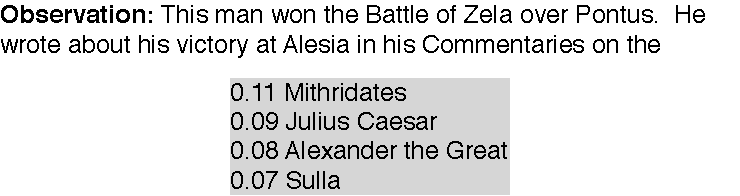
\includegraphics[width=2\linewidth]{qb/feature_ex_l_2}  \\ }
    \vspace{.5cm}
    \only<7->{ 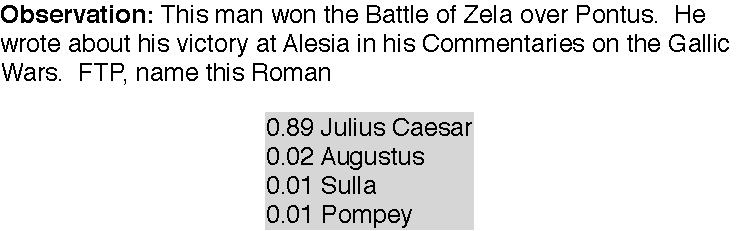
\includegraphics[width=2\linewidth]{qb/feature_ex_l_3}  \\ }


    \column{.68\linewidth}
    \vspace{-.5cm}
    \only<2->{ 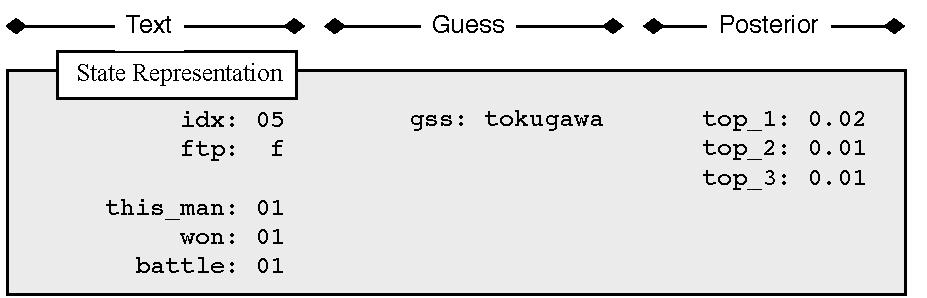
\includegraphics[width=.85\linewidth]{qb/feature_ex_r_1} \\ }
    \only<3->{ \vspace{-.5cm} \hspace{.5cm} 
\includegraphics[width=.1\linewidth]{qb/feature_ex_wait}  \\ }
    \only<5->{ 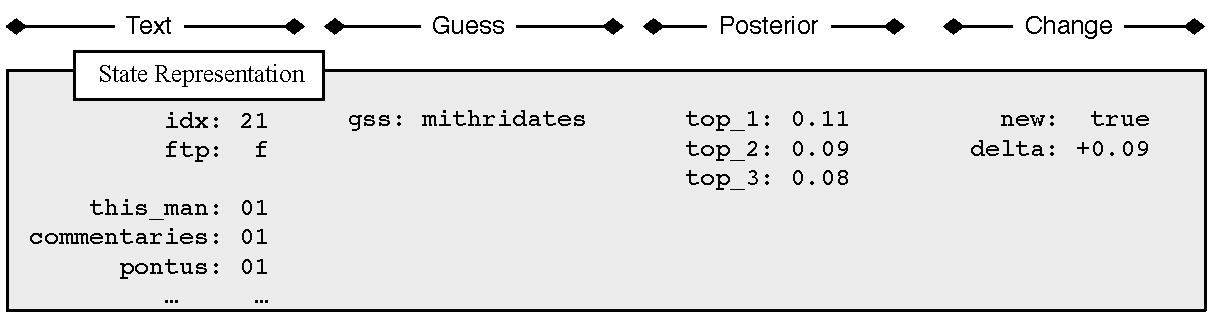
\includegraphics[width=\linewidth]{qb/feature_ex_r_2} \\ }
    \only<6->{ \vspace{-.5cm} \hspace{.5cm}
\includegraphics[width=.1\linewidth]{qb/feature_ex_wait}  \\ }
    \only<8->{ 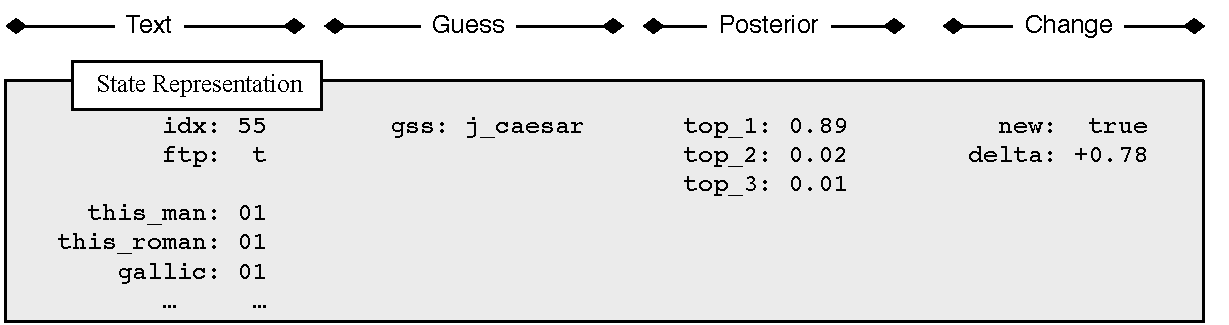
\includegraphics[width=\linewidth]{qb/feature_ex_r_3} \\ }
    \only<9->{ \vspace{-.5cm} \hspace{.5cm} 
\includegraphics[width=.1\linewidth]{qb/feature_ex_buzz}  \\ }
    \only<9->{Answer: {\bf Julius Caesar}}
  \end{columns}

\end{frame}


\begin{frame}{Add more features: DRON-concat}

  \gfxq{dron-concat}{.8}

\end{frame}


\begin{frame}{Error Analysis}

  \only<1>{\gfxq{error1}{.8}}
  \only<2>{\gfxq{error2}{.8}}
  \only<3>{\gfxq{error3}{.8}}
  \only<4>{\gfxq{error4}{.8}}
  \only<5>{\gfxq{error5}{.8}}
  \only<6>{\gfxq{error6}{.8}}
  \only<7>{\gfxq{error7}{.8}}

\end{frame}



\begin{frame}{How the shared task works}

\begin{columns}
  \column{.3\linewidth}
  \gfxq{bamber}{.5}

  \column{.65\linewidth}
  \begin{itemize}
    \item<3-> Hi! Available questions are \texttt{[1,2,3,4]}
    \item<5-> It's \texttt{Extremism}
    \item<7-> It's \texttt{in}
    \item<9-> It's \texttt{the}
    \item<11-> Got it!  You've answered Question 1 at Position
      3 with \texttt{Barry\_Goldwater}
  \end{itemize}

\end{columns}


\begin{columns}

  \column{.65\linewidth}
  \begin{itemize}
    \item<2-> I'm User~1.  I’d like to play!
    \item<4-> I’d like to hear Word~1 of Question 1
    \item<6-> I’d like to hear Word~2 of Question 1
    \item<8-> I’d like to hear Word~3 of Question 1
    \item<10-> I’d like to answer Question 1 with
      \texttt{Barry\_Goldwater}
    \end{itemize}
  \column{.3\linewidth}
  \only<2->{\gfxq{buzzer}{.5}}
\end{columns}

\end{frame}


\begin{frame}{Are there enough opportunities?}


\begin{center}
\begin{tabular}{lcccc}
\toprule
& \alert<2>{verb} & \alert<3>{voice} & \alert<4>{noun} & \alert<5>{clauses} \\
\midrule
Applicable \% & \only<2->{39.9} & \only<3->{50.0} & \only<4->{26.4} & \only<5->{4.8} \\
Accepted \% & \only<2->{22.5} & \only<3->{24.0} & \only<4->{51.2} & \only<5->{38.4} \\
\bottomrule
\end{tabular}
\end{center}

\only<2>{
\begin{itemize*}
\item[O:] {\bf They announced} that the president will restructure the division.
\item[R:] The president will restructure the division, {\bf they announced}.
\end{itemize*}
}


\only<3>{
  \begin{columns}
    \column{.4\linewidth}

    \gfxs{rewrite_input}{.9}
    \column{.55\linewidth}
    \vspace{-.5cm}
    \gfxs{rewrite_transform}{.9}
   \end{columns}
}

\only<4>{
\begin{itemize*}
  \item[O:] the e-mail server of Clinton
  \item[R:] Clinton's e-mail server
\end{itemize*}
}

\only<5>{
\begin{itemize*}
\item[O:] \pos{S}$_1$ \pos{conj} \pos{S}$_2$: We should march {\bf because} winter is coming.
\item[O:] \pos{conj} \pos{S}$_2$, \pos{S}$_1$: {\bf Because} winter is
  coming, we should march.
\vspace{1cm}
\item[R:] \pos{S}$_2$, \pos{conj'} \pos{S}$_1$: Winter is coming, {\bf because of this}, we should march.
\end{itemize*}
}


\end{frame}

\begin{frame}{}

\gfxs{rewrite_eval}{.8}
\pause
We rewrite 32.2\% of
sentences, reducing the delay from 9.9 words/seg to 6.3 words/seg per
segment for rewritten sentences and from 7.8 words/seg to 6.7 words/seg overall.

\end{frame}

\begin{frame}{How good are the translations?}

  \gfxs{tradeoff-rw-bleu}{.7}

\begin{center}
Aggressiveness based on different right probability thresholds
\cite{fujita-13}
\end{center}

\end{frame}

\begin{frame}{Why does the quality improve?}

\begin{center}
\begin{tabular}{ccccc}
\toprule
& \multicolumn{3}{c}{Translation} & \\
\cmidrule{2-4}
& \abr{gd} & \abr{rw} & \abr{rw+gd} & Gold ref \\
\midrule
\# of verbs & 1971 & 2050 & {\bf 2224} & 2731 \\
\bottomrule
\end{tabular}
\end{center}

\end{frame}

\begin{frame}{Future Steps}

  \begin{itemize}
    \item Verb prediction through argument structure \only<2->{(entity
        / coref)}
    \item Richer translation model~\cite{oda-15,cho-16}
    \item Better reward (e.g., MEANT)  \only<3->{(richer answer space)}
    \item Paraphrase database
    \item Learning from imperfect feedback  \only<4->{(player clues)}
    \item Centaur translations  \only<5->{(centaur QB)}
  \end{itemize}

\end{frame}


\end{document}
